\chapter{Implementation}
%TODO: where should we use this: problems of optical flow methods yield bad segmentations. known problems: large displacements, sharp discontinuities, accuracy for the occlusion detection.


In this chapter we explain in detail the relevant stages of our motion segmentation pipeline. We start by formulate the initial problem statement our pipeline tries to solve. Moreover, for each stage, we describe its required input data and what output it generates. Lastly, we also mention all assumptions and induced limitations for each pipeline stage. \\ \\
The problem statement our pipeline solves is defined as follows: 
Given a set of images that form a video sequence and their associated depth maps. Our goal is to separate the images into regions that form coherent and independent rigidly moving objects. \\ \\
%SHOW FIGURE OF PROBLEM STATEMENT
% INPUT: IMGS, DEPTHS, OUTPUT: SEGMENTATION
% SHOW LATER A DETAILED PIPELINE
The idea of such a segmentation is to identify and extract the meaningful rigid motions from the background. To accomplish this task we compute the optical flow on the images and use it as a guide for grouping pixel regions that belong together. Since the object motion in coherent image sequence is not independent for every frame, the optical flow depicts an ideal cue for making grouping decisions. \\ \\
Our pipeline has the following main stages:

\begin{enumerate}
\item \textbf{Dataset Preparations}: Initially, the frames of a video have to be extracted and named according to the pipeline naming conventions. If present, also the depth maps have to be named and re-normalized according to the pipeline's conventions. Optionally, a blurred version of the input images are computed by using a bilateral filter. This filtered images act as an additional, but optional cue, for a later pipeline stage. 
\item \textbf{Optical Flows}: We compute the forward- and backward-flows on our input sequence using different existing implementations. Our pipeline lets the user select a target method for generating the optical flow fields.
\item \textbf{Data Extraction}: In this stage we extract traceable feature locations in our images. Also, a mask containing all invalid tracking locations per image is computed by checking whether the the forward and backward flow correspond to each other. Optionally, depth data, flow and depth variances and color maps are extracted that are used within a later pipeline stage. 
\item \textbf{Trajectories}: We use the computed forward flows and the previously extracted traceable feature locations to perform a point tracking. A sequence of traced points form a so called trajectory. In every frame a trajectory can either be started, ended or be continued. The previously computed traceable locations act as the starting points, the forward flow is added to a traceable location and yield the tracked to position, the starting location in the next frame. Tracked to locations that land in an invalid mask location cause the tracking of a trajectory. 
\item \textbf{Affinity Matrix}: In this stage we compute the similarities between all trajectory pairs. The similarity is computed according to different metrics, which are basically a combination of various distances among overlapping trajectory parts. 
\item \textbf{Sparse Motion Segmentation}: Using the affinity matrix plus the nearest neighbouring trajectories per trajectory, we can compute its dense segmentation by either applying a spectral clustering on the affinity matrix or by reformulating the problem as a graph cut problem. Usually 
\item \textbf{Dense Segmentation}: Our pipeline allows to transform the sparse segmentation into a dense segmentation. For this purpose we consider the hole filling problem, formulating it as a convex problem and then solving it using a primal-dual approach using the sparse segmentation as the initial input.
\item \textbf{Evaluation}: Our pipeline allows to qualitatively and quantitatively evaluate the generated sparse and dense segmentations. In addition, we also can explore various parameter settings and their outcomes using different visualizers.
\end{enumerate}
In the following sections we examine and discuss each individual pipeline stage in detail. 

\section{Dataset Preparations}
The preparation of an input datasets is the very first stage of our pipeline. Initially, we have to either capture a video using one of our capturing devices or use an existing video sequence. Next, we extract all the frames from the considered video. \\ \\
In case there are also depth maps$\footnote{In case we are working with depth data, we assume that there exists one depth map per frame. Our pipeline assumes, that the values in the depth images are in meter units}$ available, they are transformed such that the value range is in meter units. For further information about the dataset conventions, read section~\ref{sec:datasets} on page~\pageref{sec:datasets}. \\ \\
Optionally, a filtered version of the input dataset images can be generated using a Bilateral Filter$\footnote{A Bilateral Filter is a non-linear, edge-preserving blur filter.}$. These filtered images can help improve the process of finding traceable candidate location as well as identifying invalid tracking locations.

\section{Computing Optical Flows}
\label{sec:impl_optical_flow}

Optical flows are used to trace coherent tacking points that form a trajectory.

Four different methods are available:
Large displacement optical flow (LDOF)
Original flow method proposed by Horn and Schunck (HS)
Semi-rigid scene flow (SRSF)
Layered RGBD flow (LRGB)


\section{Data Extraction}

% TODO formulate basic bla of dataextraction stages

Algorithm $\ref{alg:data_extraction}$ gives an overview of the involved steps in this stage.

\begin{algorithm}[H]
\caption{Data Extraction}
\begin{table}[H]
  \begin{tabular}{@{}lll@{}}
    \textbf{Input:} & Dataset Images \bf{F} \\
		& Forward- and Backward Optical Flows \bf{OF} \\
 		& Depth Images (\emph{optional}) \bf{DI} \\
    \textbf{Output:} & Traceable Feature Locations \bf{TF} \\
    & Occluded Location Masks \bf{OM}\\
    & Cie-Lab Color Images \bf{CI} \\
    & Flow Variances \bf{FV} \\
    & Depth Variances \bf{DV} \\
    
  \end{tabular} 
\end{table}
\setlength{\fboxrule}{0pt} 
\begin{boxedminipage}{1.0\textwidth}
  \begin{algorithmic}[1]
      \ForAll{$\text{frame } f \in \bf{F}$}
        \State $\text{Run Thresholded Harris Corner Detector}.$
		\State $\text{Append Sampled Features to } \bf{TF}.$
		\State $\text{Fetch } fwf,bwf \in \bf{OF} \text{ that belongs to f}.$
		\State $\text{Apply forward-backward-flow check on fwf and bwf} \bf{TF}.$
		\State $\text{Append invalid check locations to } \bf{OM}.$
		\State $\text{Apply a special variant of the bilateral filter on fwf}.$
		\State $\text{Append filtered flow to } \bf{FV}.$
		\State $\text{Transform f to CIE Lab Colorspace and append it to } \bf{CI}.$
		\State $\text{Fetch } df \in \bf{DI} \text{ that belongs to f}.$
		\State $\text{Apply a 2-pass special variant of the bilateral filter on } df$
		\State $\text{Append the filtered depth to } \bf{DV}$
      \EndFor
  \end{algorithmic}
  \end{boxedminipage}
  \vskip1.5pt
\label{alg:data_extraction}
\end{algorithm}

\subsection{Tracking Candidates}
Explain purpose of the tracking candidates. \\ \\
Figure $\ref{fig:tracable_candidates}$ illustrates the feature locations that can be used in the tracking stage of the pipeline. For a given image as shown in subfigure $\ref{fig:c14_f1_cand}$ we initially compute interseting features using by applying a Harris corner detector onto it. The result is shown in figure $\ref{fig:c14_cand_corners}$. We filter weak corner candidates by thresholding too weak corners. A detailed explanation how this thresholding works is described in the appending in section $\ref{sec:corner_thresholding}$ on page $\pageref{sec:corner_thresholding}$.

 The remaining corners form a boolean selection mask as shown in figure $\ref{fig:c14_cand_dense}$. Finally, to avoid oversampling, we further reduce the number of samplings by only taking every $n-th$ sample location. The final tracking canidates are shown in figure $\ref{fig:c14_cand_sparse}$, illustrated as red dots, overlaid on top of the initial input image.
\begin{figure}[H]
\begin{center}
\subfigure[Input Image]{
   \includegraphics[width=0.48\linewidth] {implementation/candidates/01}
   \label{fig:c14_f1_cand}
}
\subfigure[Sparse Candidates]{
   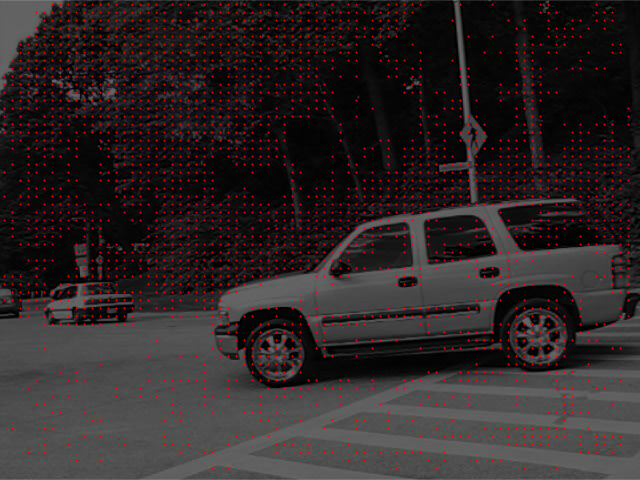
\includegraphics[width=0.48\linewidth] {implementation/candidates/candidates_sparse}
   \label{fig:c14_cand_sparse}
}
~
\subfigure[Harris Corners]{
   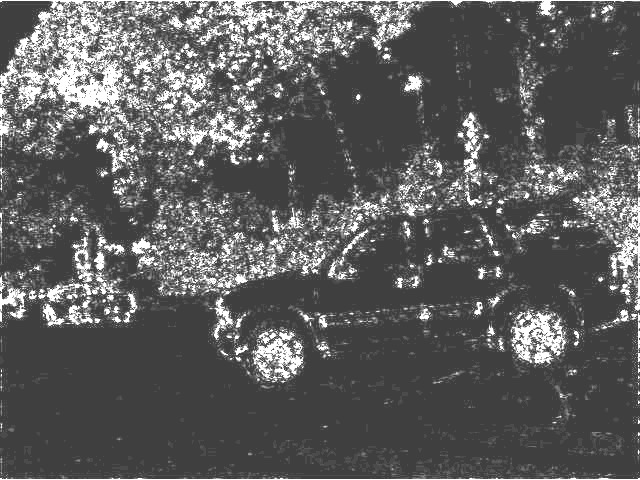
\includegraphics[width=0.48\linewidth] {implementation/candidates/out_corners}
   \label{fig:c14_cand_corners}
}
\subfigure[Dense Candidates]{
   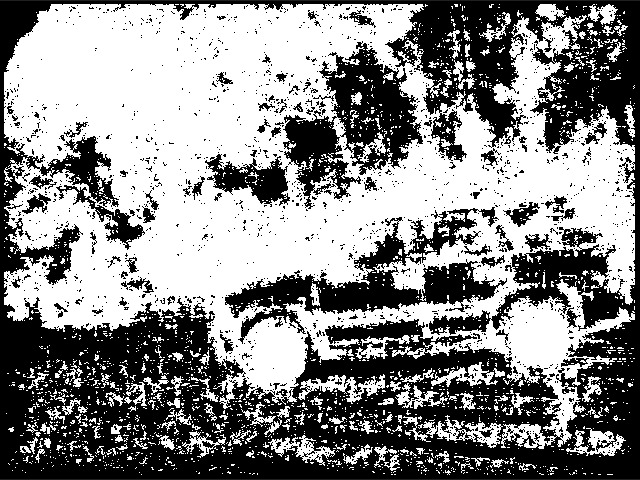
\includegraphics[width=0.48\linewidth] {implementation/candidates/c14_f1_candidates}
   \label{fig:c14_cand_dense}
}
\end{center}
\caption[Tracking Candidates]{A visualization of the tracking candidates extraction stages. For a given input image as shown in subfigure $\ref{fig:c14_f1_cand}$ we want to compute a sparse set of traceable feature locations as shown in subfigure $\ref{fig:c14_cand_sparse}$.}
\label{fig:tracable_candidates}
\end{figure}


a set of points is initialized in the first video frame.
principally, every pixel location could be used. however, homogeneous areas can be problematic for the optical flow. therefore, only reliable points are kept and we remove points that doe not show any structure in their vicinity based on the smaller eigenvalue of the structure tensor. 

for efficiency reasons, we spatially subsample the initial points.
factors larger than 12 lose details as there are not enough points to cover small object parts. on the other hand, factors smaller than 6 waste computation time as smaller objects tend to get smoothed away. 

An illustration of different sampling rates is shown in figure $\ref{fig:sampling_rate_candidates}$.
\begin{figure}[H]
\begin{center}
\subfigure[Extreme Oversampling]{
   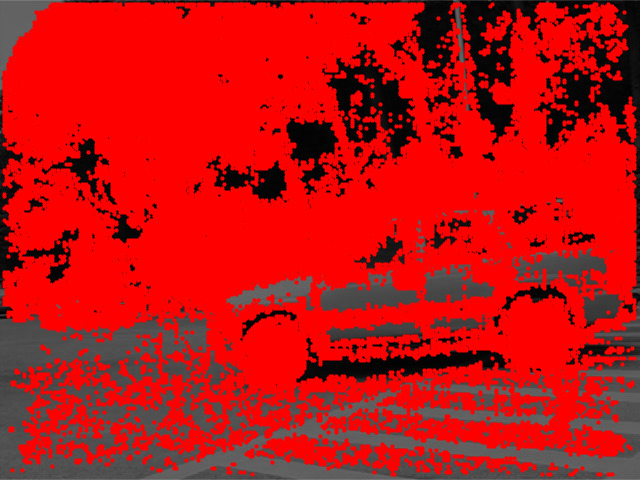
\includegraphics[width=0.48\linewidth] {implementation/candidates/sr_2}
   \label{fig:c14_extreme_oversampling}
}
\subfigure[Oversampling]{
   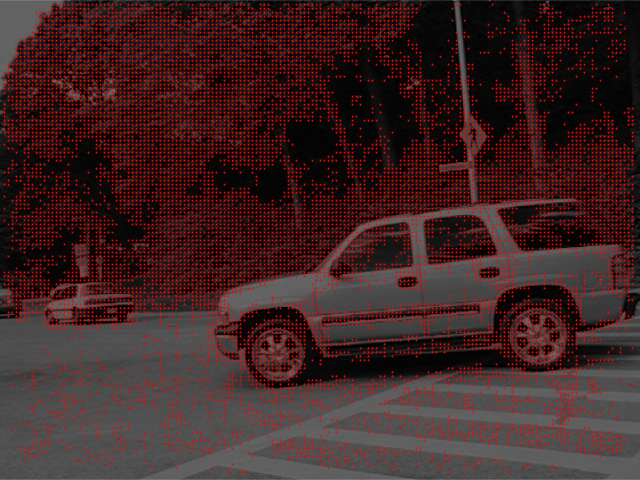
\includegraphics[width=0.48\linewidth] {implementation/candidates/sr_4}
   \label{fig:c14_oversampling}
}
~
\subfigure[Ideal Sampling Rate]{
   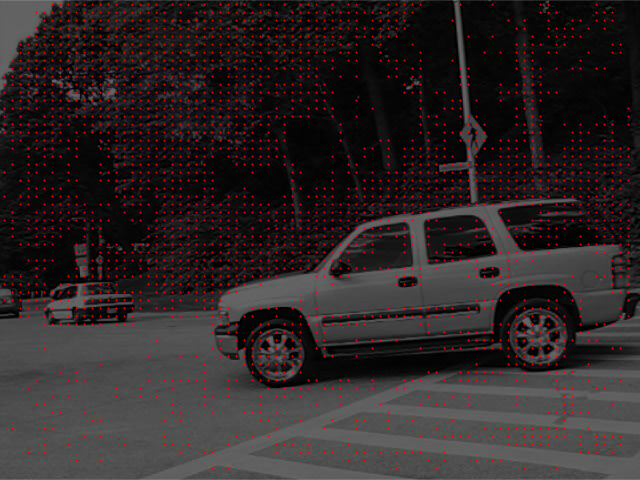
\includegraphics[width=0.48\linewidth] {implementation/candidates/sr_8}
   \label{fig:c14_ideal_sampling}
}
\subfigure[Undersampling]{
   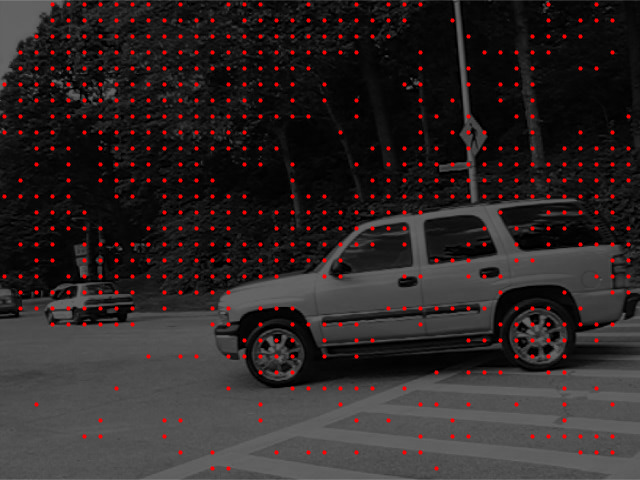
\includegraphics[width=0.48\linewidth] {implementation/candidates/sr_16}
   \label{fig:c14_undersampling}
}
\end{center}
\caption[Density Of Candidates For Different Sampling Rates]{A visualization of different sampling rates of tracking candidates}
\label{fig:sampling_rate_candidates}
\end{figure}


Traceable candidate locations are obtained by applying a Harris Corner Detector on the input image. 
Features that are identified as corners are a viable option for starting a trajectory tracking.

in addition, a boolean grid with a certain cell size is applied to the candidates, acting as a selection mask. This reduces the number of tracking candidates (spacial subsampling) drastically and makes the sampling sparser.


mention how invalid regions are computed: occluded regions.

\begin{figure}[H]
\begin{center}
\subfigure[All Dense Candidates]{
   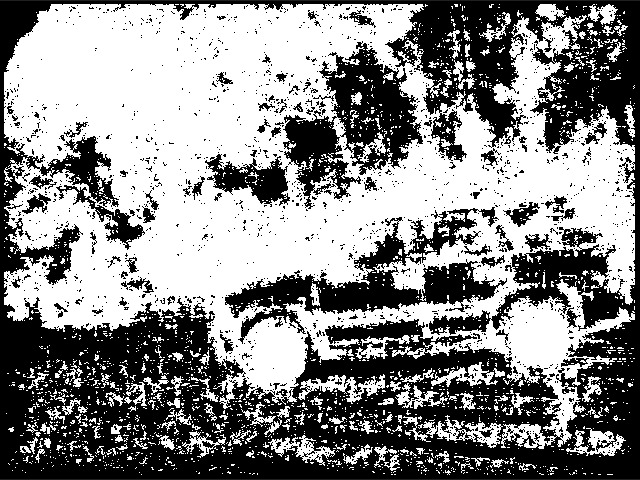
\includegraphics[width=0.48\linewidth] {implementation/candidates/c14_f1_candidates}
   \label{fig:c14_f1_cand_dense_2}
}
\subfigure[Strict Dense Candidates]{
   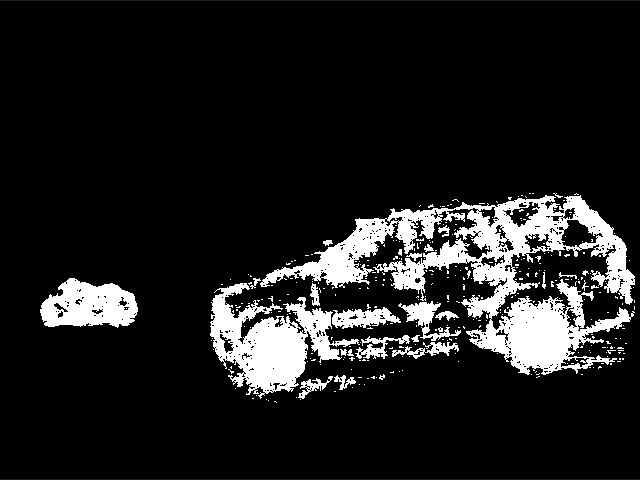
\includegraphics[width=0.48\linewidth] {implementation/candidates/strict_dense_candidates}
   \label{fig:c14_cand_dense_strict}
}
\end{center}
\caption[Strict Dense Candidates]{A visualization of the final dense traceable features.}
\label{fig:tracable_candidates_strict}
\end{figure}







\subsection{Occlusion detection}
idea: stop tracking points as soon as a point gets occluded.

in tracking, occlusion is usually detected by comparing the appearance of the local neighborhood of the tracked point over time. in contrast, we detect occlusions by verifying the consistency of the forward and the backward flow.

Occlusion is detected by applying the backward flow to a continued tracked point and checking whether that resulting point has the same origin as the actual tracked from position. Figure $\ref{fig:occlusion_detection}$ illustrates this concept of occlusion detection.
%TODO create figure showing: point in frame 1 gets  tolerance interval
\begin{figure}[H]
\begin{center}
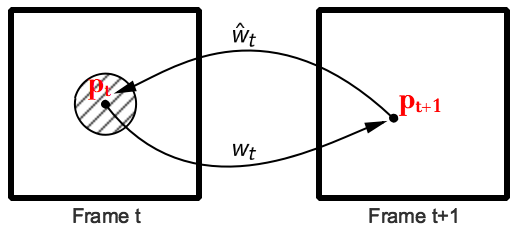
\includegraphics[width=0.6\linewidth] {implementation/occlusion/occ_det}
\end{center}
\caption[Occlusion Detection]{Conceptual illustration of occlusion detection. For any tracking candidate we apply its corresponding forward flow to find its position in the next frame. From there, we look-up its backward flow and apply it on the tracked to position. If we land close to the point in the original tracked from frame, we say, that the point is not occluded and otherwise we call the point occluded.}
\label{fig:occlusion_detection}
\end{figure}
In non-occluded case, the backward flow vector points in the inverse direction of the forward flow vector. if this consistency required is not satisfied, the point is either getting occluded at frame $t+1$ (the next frame) or the flow was not correctly estimated. both are good reasons to stop tracking this point at frame $t$. Since there are always some small estimation errors in the optical flow, there is a small tolerance interval granted. The formula used to decide when a point is not occluded is given in equation $\ref{eq:occlussion_error_tol}$.
\begin{equation}
\begin{aligned}
& \forall p_t \in \text{Frame t}:	\norm{\hat{p_t}-p_t}_2^2 < \epsilon \norm{\hat{w}_t - w_t}_2^2 + b \\
& \text{where } \hat{p_t} = p_{t+1} + \hat{w_t} \text{ with } p_{t+1} = p_t + w_t
\end{aligned}
\label{eq:occlussion_error_tol}
\end{equation} \\
Occlusion comes with the opposite phenomenon disocclision or scaling. to fill these areas not covered by trajectory yet, new trajectories are initialized, in empty areas in each new frame using the same strategy as for the first frame.

\begin{figure}[H]
\begin{center}
\subfigure[Input Image]{
   \includegraphics[width=0.48\linewidth] {implementation/occlusion/01}
   \label{fig:c14_f1_occ}
}
\subfigure[Occluded Regions]{
   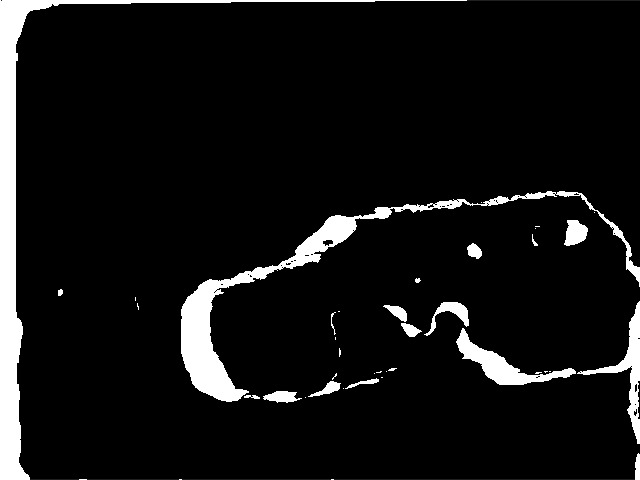
\includegraphics[width=0.48\linewidth] {implementation/occlusion/invalid_regsions}
   \label{fig:c14_invalid_regions}
}
\end{center}
\caption[Occluded Regions]{A visualization of the occluded regions. Invalid, occluded regions are colored in white illustrated as shown in subfigure $\ref{fig:c14_invalid_regions}$.}
\label{fig:invalid_regions}
\end{figure}

the color values are stored as CIE lab color images.

\subsection{Flow Variance}

In a later stage in our pipeline, we will compute differences between different optical flow field locations. Since our optical flows may contain noise, especially along motion boundaries, we have to make our pipeline robust to these negative influence of noise. In particular, when taking the difference between two noisy flow locations, the noise level can get amplified. The purpose of this section is to describe a method how to normalize flow differences. 

An simple, but initial first idea would be to smooth the computed flow fields, to reduce the noise level along the boundaries. A commonly used approach to blur an image is to convolve the image with a Gaussian kernel as defined in equation $\ref{eq:gaussian_filter}$.
\begin{equation}
	G_{\sigma}\left( x \right) = \frac{1}{2 \pi \sigma^2} e^{-\frac{x^2}{2 \sigma^2}}
\label{eq:gaussian_filter}
\end{equation}
However, filtering the flows directly is not the best choice. The reason for this is based on the fact that a Gaussian filter acts as a low-pass filter. Thus, after applying this kernel, many details in the flow, such as motion boundaries, will be washed out or will be removed completely. \\ \\
Another blur filter, which addresses the issue of smoothing out edges, is the so called Bilateral Filter $\textbf{BF}$. Similar to the Gaussian Convolution, this filter also computes a weighed average of an image, but the same time takes into account the variation of intensities to preserve edges. 

Let $\bf{I}$ denote an image and $\bf{p}$ one of its pixels. The neighborhood pixels of $\bf{p}$ are denoted by $\mathcal{N}_p$. Then, the Bilateral filter $\textbf{BF}$ can be defined as described in equation $\ref{eq:bilateral_filter}$.
\begin{equation}
	\textbf{BF} \left\{ \bf{I}_{\bf{p}} \right\} = \frac{1}{W_{\bf{p}}} \sum_{\bf{q} \in \mathcal{N}_p} w_{\bf{p}, \bf{q}} \left( \bf{I} \right) \bf{I}_{\bf{q}}
\label{eq:bilateral_filter}
\end{equation}
Note that $w_{\bf{p}, \bf{q}}$ denotes the weight between the pixels $\bf{p}$ and $\bf{q}$, whereas the term $W_{\bf{p}}$ defined in equation $\ref{eq:bilateral_filter_weights}$ is the sum of all weights between a fixed pixel $\bf{p}$ and its neighbors.

\begin{equation}
	w_{\bf{p}, \bf{q}} \left( \bf{I} \right) = G_{\sigma_s} (\norm{\bf{p} - \bf{q}}) G_{\sigma_r} (\bf{I}_{\bf{p}} - \bf{I}_{\bf{q}}) 
\label{eq:bilateral_filter_neighbor_weight}
\end{equation}

The weight in equation $\ref{eq:bilateral_filter_neighbor_weight}$ has a spatial component $G_{\sigma_s} (\norm{\bf{p} - \bf{q}})$ as well as it considers the intensity range $G_{\sigma_r} (\bf{I}_{\bf{p}} - \bf{I}_{\bf{q}})$.

\begin{equation}
	W_{\bf{p}} \left( \bf{I} \right) = \sum_{\bf{q} \in \mathcal{N}_p} w_{\bf{p}, \bf{q}} \left( \bf{I} \right)
\label{eq:bilateral_filter_weights}
\end{equation}
Instead of using a filtered flow field, we go for another, more robust idea. Imagine we would know the error of the computed flows. Then, by using the variance of the field, we directly could address the error by normalizing the flow value by its corresponding variance value. Since we do not know the actual error, we have to define a good estimator of the flow variance. \\ \\
Let $\bf{q}_p$ denote a vector containing all neighbors of pixel $\bf{p}$ and $\bf{w}_p$ is the vector consisting of all weights computed using equation $\ref{eq:bilateral_filter_neighbor_weight}$. Mathematically, this can be formulated as the follows:
\begin{equation}
\begin{aligned}
& \bf{q_p} = \left( q_1, \dots, q_{|\mathcal{N}_p|} \right) \\
& \bf{w_p} = \left( w_{p, q_1}, \dots, w_{p, q_{|\mathcal{N}_p|}} \right) \\
& \text{where } \forall q_k \in \mathcal{N}_p
\end{aligned}
\label{eq:bilat_weight_components}
\end{equation}

The definitions from equation $\ref{eq:bilat_weight_components}$ allow us to define an expected value of pixel $\bf{p}$.

\begin{equation}
	\mathbf{E} \left[ \bf{p} \right] = \frac{\bf{w}_{p}^{T} \bf{q}_p}{\norm{\bf{w}_{p}}}
\end{equation}

For a given optical flow $\bf{F} = (\bf{F_u}, \bf{F_v})$ we can compute its variance by the definition stated in equation $\ref{eq:flow_var_opt_flow}$.
\begin{equation}
	\mathbf{Var} \left[ \bf{F} \right] = \frac{1}{2} \left( \mathbf{Var} \left[ \bf{F_u} \right] + \mathbf{Var} \left[ \bf{F_v} \right] \right)
\label{eq:flow_var_opt_flow}	
\end{equation}

STATE MEANING

\begin{figure}[H]
\begin{center}
\subfigure[Flow Field]{
   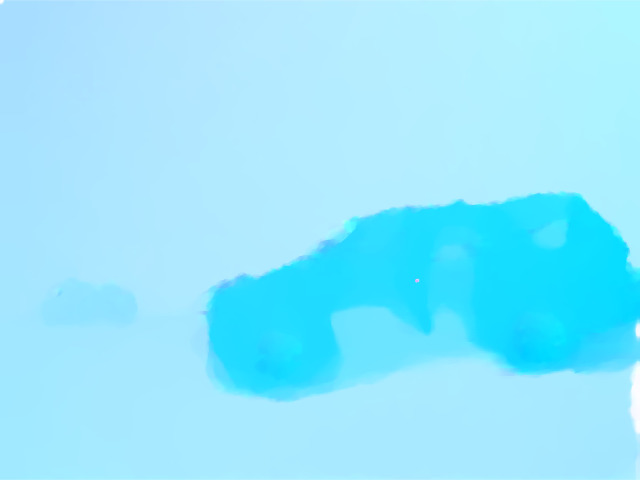
\includegraphics[width=0.48\linewidth] {implementation/flow_var/ff_c14_1}
   \label{fig:c14_fv_flow}
}
\subfigure[Variance Field]{
   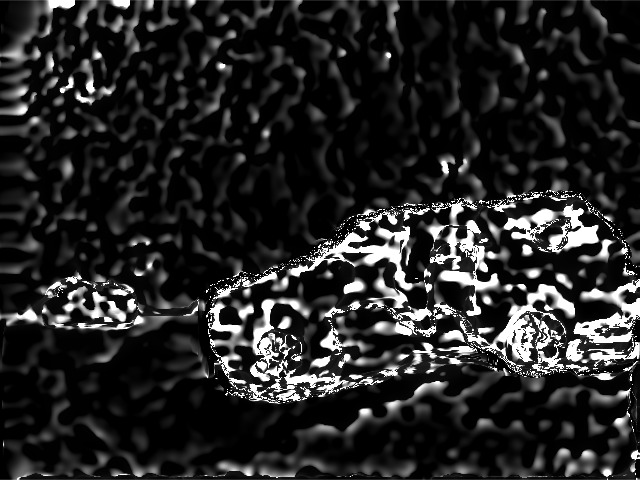
\includegraphics[width=0.48\linewidth] {implementation/flow_var/fv_c14_1}
   \label{fig:c14_fv_var}
}
\end{center}
\caption[Flow Variance]{Visualization of the flow variance computed by applying a bilateral filter on the optical forward flow.}
\label{fig:flow_variance}
\end{figure}


flow estimation can be noisy for various reasons and the problem is that the nois is often proportional to the magnitude of the absolud flow. thus using a simple flow difference as ameasure will constantly underestimate the simmilarity between heigh magnitude flow. 

Lets assume 

\begin{equation}
\begin{aligned}
\colvec{u_1}{v_1} = f + \colvec{x_1}{y_1} \\
\colvec{u_2}{v_2} = f + \colvec{x_2}{y_2}
\end{aligned}
\label{eq:def_flow_tracking}	
\end{equation}

where f is the true flow and 
\begin{equation}
	\colvec{x_1}{y_1} \sim \colvec{x_2}{y_2}
\end{equation}

Let us assume, that the random variables $x_1$ and $x_2$ are i.i.d. distributed having a zero mean and a variance $\sigma_x^2$, $x_1$ and $x_2$ respectively, i.e.

\begin{equation}
\begin{aligned}
x_1 \sim x_2 (0, \sigma_x^2) \\
y_1 \sim y_2 (0, \sigma_y^2
\end{aligned}
\label{eq:def_flow_tracking}	
\end{equation}

\begin{equation}
\begin{aligned}
\mathbf{E} \left[ \norm{\colvec{u_1}{v_1} - \colvec{u_2}{v_2}} \right]
& = \mathbf{E} \left[ (u_1 - u_2)^2 \right] + \mathbf{E} \left[ (v_1 - v_2)^2 \right] \\
& = \mathbf{E} \left[ u_1^2 - 2 u_1 u_2 + u_2^2 \right] + \mathbf{E} \left[ v_1^2 - 2 v_1 v_2 + v_2^2 \right] \\
& = \mathbf{E} \left[ x_1^2 \right] + \mathbf{E} \left[ x_2^2 \right] + \mathbf{E} \left[ y_1^2 \right] + \mathbf{E} \left[ y_2^2 \right] \\
& = 2 \left( \sigma_x^2 + \sigma_y^2 \right)
\end{aligned}
\label{eq:flow_variance_formula}	
\end{equation}
In the last step of equation $\ref{eq:flow_variance_formula}$ we used the abbreviation $\sigma_x^2$ which denotes the variance of the optical flow along its $x$ direction. In this derivation we exploited the fact that $x_1$ and $x_2$ are independent random variables, $y_1$ and $y_2$ respectively. Hence, the term $\mathbf{E} \left[ x_1 x_2\right]$ yields the value zero.


depth fields
color values
depth field variances.



\section{Trajectories}
As discussed earlier, motion is a spatially and temporal coherent visual cue. This key insight tells us that motion is not frame-wise independent. Hence, we have to extract the whole motion history of every frame location and feed it to a particular segmentation method in order to produce viable motion groupings. To build the history of a point we track it to its successor frames using the optical flow. Such a ordered list of tracked to points is called trajectory. Finally, the set of all possible trajectories forms the seeked motion history. In this section we explain in detail the required steps to generate such trajectories and their 3d version using camera calibration data.

\subsection{Point tracking}
Every point in frame $t$ can be tracked to the next frame $t+1$ by using the optical flow field $w_t$ that belongs to frame $t$. 	In principle, any optical flow method can be used. Our implementation supports various flow methods$\footnote{In general, our pipeline supports any flow method that can produce .flo files. However, the follwoing methods are directly supported: the \textit{ldof}, \textit{hs}, \textit{srsf} and \textit{lrgbd} flow methods}$. Please refer to section $\ref{sec:impl_optical_flow}$ on page $\pageref{sec:impl_optical_flow}$ to get a detailed list and description. Algorithm $\ref{alg:point_tracking}$ \\ \\

\begin{algorithm}[H]
\caption{Point Tracking}
\begin{table}[H]
  \begin{tabular}{@{}lll@{}}
    \textbf{Input:} & Tracking candidates $\textbf{TC}$ \\
    	& Forward Flow fields $\textbf{F}$ \\
        & Occluded Regions $\textbf{OR}$ \\
	\textbf{Output:} & Trajectories $\textbf{TC}$
  \end{tabular} 
\end{table}
\setlength{\fboxrule}{0pt} 
\begin{boxedminipage}{1.0\textwidth}
  \begin{algorithmic}[1]
  	\State $\text{Load tracking candidates TC of first frame} f_1$
  	\State $\text{Load forward flow } \text{ff}_1 \text{ of first frame } f_1.$
  	\State $\text{Initalize a PointList } \bf{PL} \text{ containing all tracked to positions}.$
  	\ForAll{$\text{trackingCandidate.position } p \in TC\left( f_1 \right)$}
  		\State $\text{Fetch flow vector fv} = \textbf{F} \left( f_1, p \right)$
  		\State $\text{Compute the tracked to position: } tp = p + fv$
  		\State $\text{Append tp to TC}$
    \EndFor
    \State $\text{Append TC to the Tracking Candidates that belong to Frame 2}.$
  	\ForAll{$\text{Frame } f \in \{ \text{Frame}_2,\dots, \text{Frame}_n\}$}
  	  	\State $\text{Load tracking candidates TC of first frame} f$
  		\State $\text{Load forward flow } \text{ff} \text{ of frame } f.$
  		\State $\text{Initalize a PointList } \bf{PL} \text{ containing all tracked to positions}.$
  		\ForAll{$\text{trackingCandidate.position } p \in TC\left( f \right)$}
  			\State $\text{Fetch flow vector fv} = \textbf{F} \left( f, p \right)$
  			\State $\text{Compute the tracked to position: } tp = p + fv$
  			\State $\text{Append tp to TC}$
    	\EndFor
    	\State $\text{Append TC to the Tracking Candidates that belong to next frame}.$
    \EndFor
  \end{algorithmic}
  \end{boxedminipage}
  \vskip1.5pt
\label{alg:point_tracking}
\end{algorithm}
$\newline$
Initially, we load all the extracted Harris corner feature locations that belong to the first dataset frame and its corresponding forward flow field. For each such feature location, we lookup its value in the flow field. Next, we add this looked-up flow vector to currently considered feature image coordinate. The result is the \textit{tracked to} position within the second frame. If this computed tracked to position is not occluded, we keep it. Otherwise we discard it. Deciding whether or not a location is occluded is done by performing a lookup in the occlusion mask. Moreover, points that land outside valid image locations are discarded. \\ \\
After processing the first frame, we continue with tracking points in the next frame. This time we not only have to track the extracted Harris features, but we also have to continue every \textit{tracked to} position from the previous iteration. To fill disoccluded areas not covered by trajectory yet, new trajectories are initialized, in empty areas in each new frame using the same strategy as for the first frame. \\ \\
The set of all these locations is processed the same way as described as the points in the initial stage. We repeat this procedure until we visited every dataset frame. \\ \\
Again, please note that tracking data has to be stopped as soon as a point gets occluded. otherwise, the point trajectory will share the motion of two different objects. \\ \\
Finally, figure $\ref{fig:cars_trajectories}$ gives an impression of an actual point tracking, showing the resulting trajectories on the \textit{cars} dataset. As we can see, points tracked in the same moving objects exhibit coherent trajectories.
\begin{figure}[H]
\begin{center}

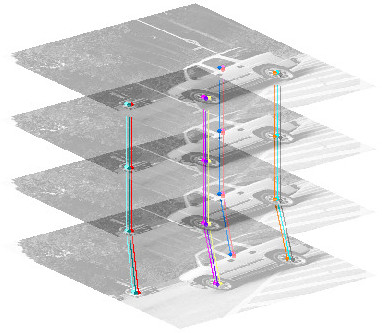
\includegraphics[width=0.65\linewidth] {implementation/trajectories/cars_trajectories_4_sel}
\end{center}
\caption[Trajectories]{Exemplary trajectories tracked in the cars dataset shown in different color. The tracking points exhibit the same color as the trajectory the belong to. The tracking points are plotted as thick dots.}
\label{fig:cars_trajectories}
\end{figure}

\subsection{Transformation to 3d points}
\label{subsection:transform_to_3d_points}
Ultimately, our pipeline should be able to work with 3d data. To enable this, we have to make use of the extracted depth map and use their information in order to transform the 2d trajectory points to 3d points in space. Ideally, the distances, computed to define an affinity measure between trajectories, should be more accurate. 

Given the principal point $p = \left(p_x, p_y \right)$ and the focal lengths $\left(f_x, f_y \right)$ we can compute the following homogeneous transformation:
\begin{equation}
\colvec[f_x X + Z p_x]{f_y Y + Z p_y}{Z} =
\begin{bmatrix}
f_x & 0 & p_x & 0 \\
0 & f_y & p_y & 0 \\
0 & 0 & 1 & 0
\end{bmatrix}
\begin{pmatrix}
X \\
Y \\
Z \\
1
\end{pmatrix}
\end{equation}

In the following, let us assume $d \equiv z$. Then

\begin{equation}
	\colvec[X]{X}{Z} \mapsto \left( \frac{f_x x}{d} + p_x, \frac{f_y y}{d} + p_y \right)^T
\end{equation}

since

\begin{equation}
\begin{aligned}
	d \left( \frac{x - p_x}{f_x} \right) = \hat{x} \Leftrightarrow \frac{\hat{x}}{d} f_x + p_x = x \\
	d \left( \frac{y - p_y}{f_y} \right) = \hat{y} \Leftrightarrow \frac{\hat{y} f_y}{d} + p_y = y 
\end{aligned}
\label{eq:depth_tranfomation}
\end{equation}.

For given pixel coorinates $\left( x,y \right)$ that indicate image locations, we want to transform them into camera coordinates, using depth maps, by applying equation $\ref{eq:depth_tranfomation}$.

given the extrinsic and intrinsic camera calibration data,

\begin{equation}
\begin{aligned}
	\text{Camera}^{depth} : \left( p^d = (p_x^d, p_y^d), f^d = (f_x^d, f_y^d)\right) \\
	\text{Camera}^{color} : \left( p^c = (p_x^c, p_y^c), f^c = (f_x^c, f_y^c)\right) \\
	\textbf{E} : \text{Camera}^{depth} \rightarrow \text{Camera}^{color}
\end{aligned}
\label{eq:calib_data}
\end{equation}.

Steps to transform 2d image locations $\left( u, v \right)$ to 3d positions $\left( x, y, z \right)$ using the camera calibration data defined as in equation $\ref{eq:calib_data}$. Furthermore, let the depth value d $\in$ $\bf{D}$. Then we have to perform the following transformations steps:

\begin{enumerate}
\item Transform image location onto depth camera space
\begin{equation}
	\forall (u, v), \forall d = \textbf{D}(u,v): \colvec[\frac{u - p_x^d}{f_x^d} d]{\frac{v - p_y^d}{f_y^d} d}{d} = \colvec[x]{y}{z} \equiv \bf{p}
\end{equation}
\item Align depth camera on color camera by appling the extrinsic matrix $E$:
\begin{equation}
	\forall p: \hat{p} \equiv \colvec[\hat{x}]{\hat{y}}{\hat{z}} =  E p
\end{equation}
\item transform onto color camera
\begin{equation}
	\forall \hat{p} : \left( \hat{u}, \hat{v}\right) = \colvec{\frac{\hat{x}}{\hat{z}} f_x^c + p_x^c}{\frac{\hat{y}}{\hat{z}} f_y^c + p_y^c}
\end{equation}
\end{enumerate}



\section{Affinity Matrix}
In this section we describe how we compute the so called affinity matrix, which is later used to compute the actual motion segmentation.

Trajectories of longer videos are asynchronous, i.e. cover different temporal windows in a shot. the set of points that are tracked across the whole scene is small or empty due to occlusion and disocclusion. a measurement matrix that takes the coordinates of the tracked points in all frames, as used by the multi-body factorization and subspace methods, will have many missing entries. therefore, such a measurement matrix is avoided. rather, pairwise affinities between trajectories are computed. this only requires some trajectories to have some temporal overlap.

we define affinities between all pairs of trajectories that share at least a common frame. In the following we denote the tracking points in these shared frames as overlapping parts.

Hence, as the very first step our pipeline fetches the previously extracted trajectories to form every possible pair combination. For each trajectory pair different distance values are computed and combined according to an initially by a pre-specified run-mode. More precisely, our pipeline computes the following three distances between overlapping trajectory segments:

\begin{itemize}
  \item The spatial distance $d_{\text{spatial}}$: Trajectories that belong to the same object are usually spatially close to each other.
  \item the color distance $d_{\text{color}}$: within a certain object region, associated trajectories are tracked at locations that have a similar color value.
  \item the motion distance $d_{\text{motion}}$: according to the gestalt principle, for each pair of trajectories at the time instant where the motion is maximally different, we can conclude, that the two points do not belong to the same object.
\end{itemize}

% ADD FIGURE SHOWING THE DISTANCES

The spatial distance is simply the average distance between the overlapping pair segments according to the euclidean norm. For computing the color distance we do the following: For every overlapping tracking point of any pair, we lookup the color value in its corresponding frame. Then, we compute the distance between the looked-up color values by transforming the color values to the $\text{CIE l*a*b}$ colorspace$\footnote{This transformation enables us to use the l2 norm in order to compute color distances.}$ and then applying the l2 norm. We finally compute the average of these color distances which is equals $d_{\text{color}}$. 

Lastly, some insight into how the motion distance is computed.


There are two main setting a user has to specify preliminarily: Whether or not depth cues should be used and which kind of similarity measure should be used. 

Both options have a large impact on the final outcome of the affinity matrix. When enabling depth cues, all available depth fields are loaded into the pipeline. In combination with the depth- and color-camera calibration data, this enables the pipeline to compute the three dimensional version of each traced trajectory point, analogous as described in the previous subsection $\ref{subsection:transform_to_3d_points}$ on page $\pageref{subsection:transform_to_3d_points}$. This 3d positions are then used for computing the spatial distance between the overlapping parts of any trajectory pair. \\ \\
Our pipeline basically supports two distance combination methods: Either it combines them by calculating the weighted sum of the distance values or it multiplies all the distances. Depending on the used combination strategy, different segmentation methods will later be used. Summed distances can only be used in combination together with the Kernighan-Lin segmentation method whereas the product of distances can be either used in our spectral clustering- or min-cut segmentation method$\footnote{The reason for this limitation is due to the fact that the summed distance method may yield negative affinities since some weights are negative.}$.

All possible modes are listed in figure $\ref{fig:affinity_modes}$.
\begin{figure}[H]
\begin{center}
   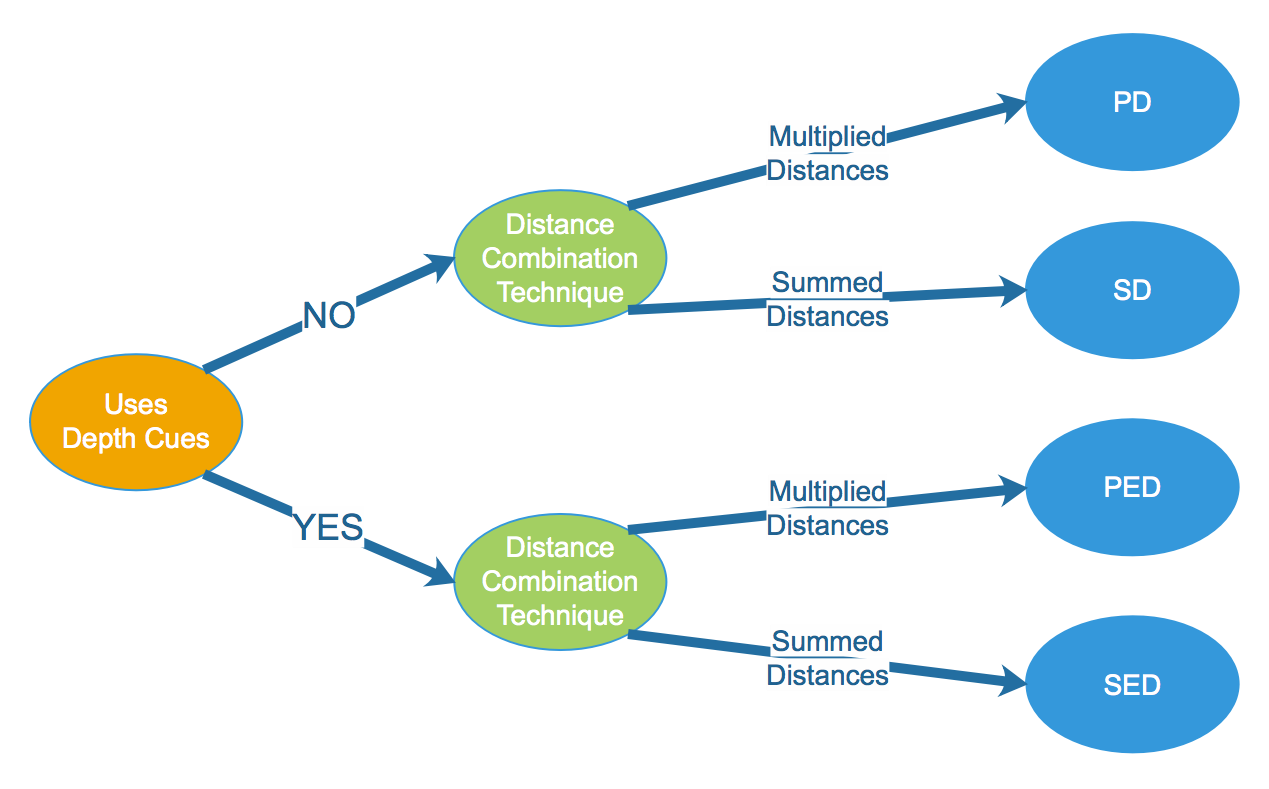
\includegraphics[width=0.7\linewidth] {implementation/affinities/modes}
   \label{fig:cars_w}
\end{center}
\caption[Affinity Pipeline Modes]{foobar}
\label{fig:affinity_modes}
\end{figure}

%TODO Mention the available runtime combinations and their abbreviations


When combining the distances by taking their product, we c
$\ref{sec:trajectory_affinities}$ on page $\pageref{sec:trajectory_affinities}$.

Moreover a user also has to assign which dataset should be used for.  

 
Apart from generating the affinity matrix our pipeline also extracts the nearest neighboring trajectories for every trajectory.



\begin{figure}[H]
\begin{center}
\subfigure[Similarities Car Forground]{
   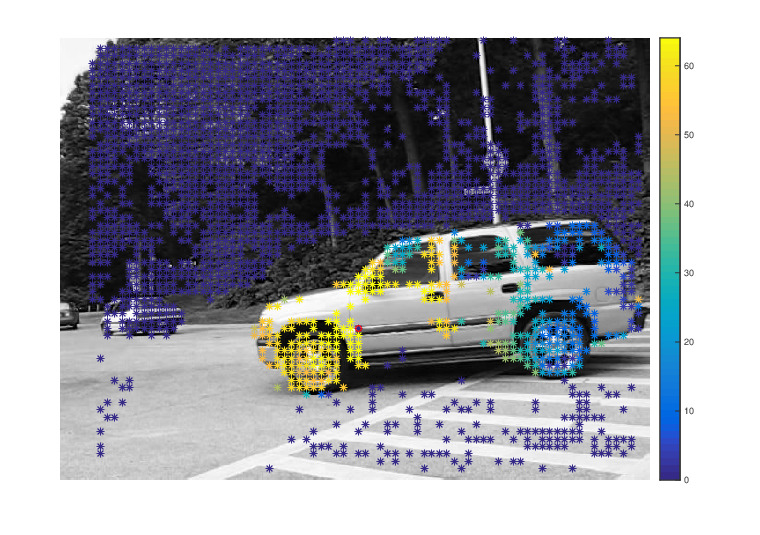
\includegraphics[width=0.48\linewidth] {implementation/affinities/cars/fc}
   \label{fig:cars_a}
}
\subfigure[Similarities Car Background]{
   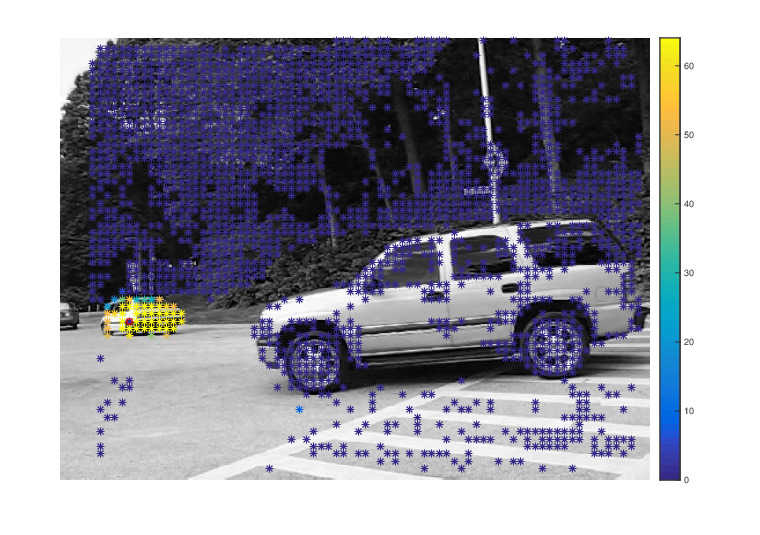
\includegraphics[width=0.48\linewidth] {implementation/affinities/cars/cb}
   \label{fig:cars_b}
}
~
\subfigure[Similarities Woods]{
   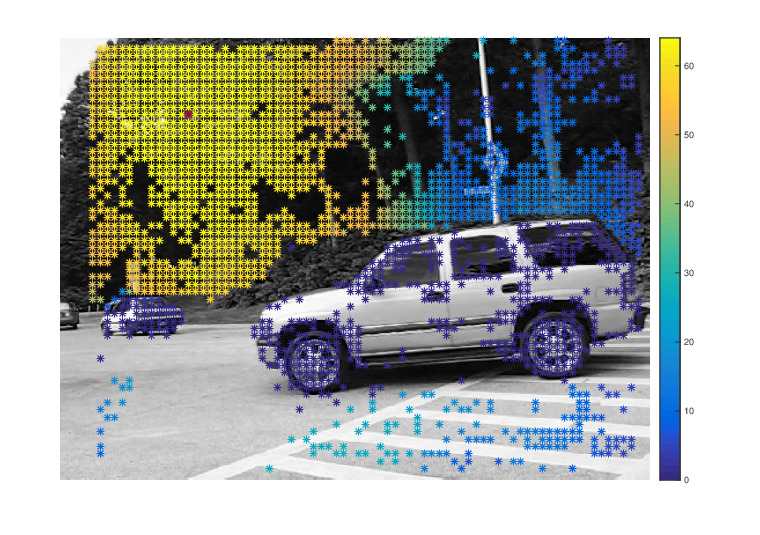
\includegraphics[width=0.48\linewidth] {implementation/affinities/cars/woods}
   \label{fig:cars_c}
}
\subfigure[Similarities Street]{
   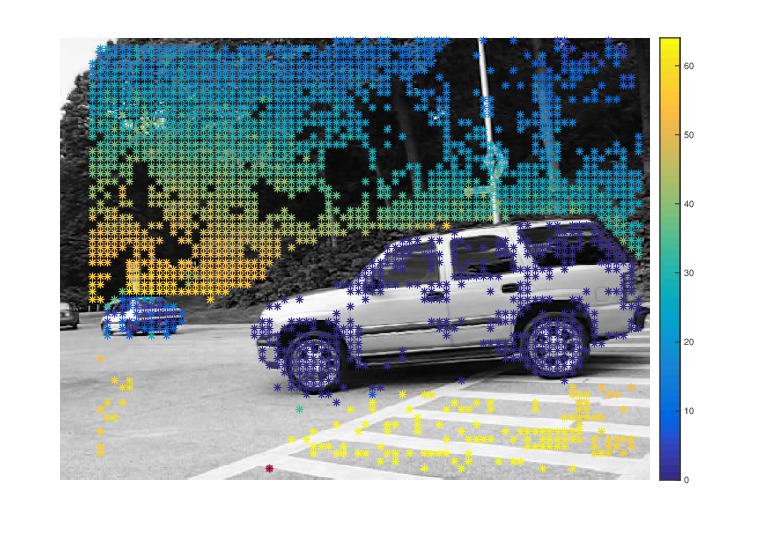
\includegraphics[width=0.48\linewidth] {implementation/affinities/cars/street}
   \label{fig:cars_d}
}
\end{center}
\caption[Trajectory Affinities]{Visualization of affinities among trajectories and the structure of the matrix $W$.}
\label{fig:cars_affinities}
\end{figure}


\begin{figure}[H]
\begin{center}
   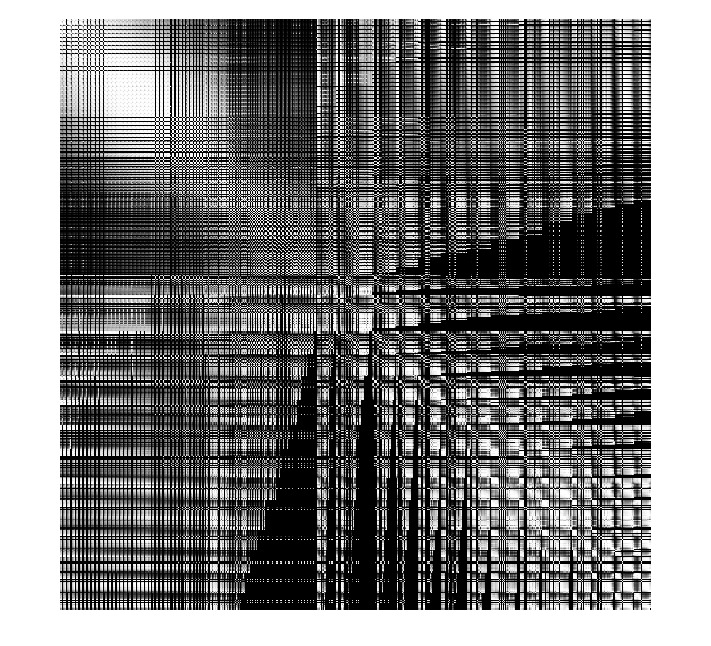
\includegraphics[width=0.65\linewidth] {implementation/affinities/cars/cars_w}
   \label{fig:cars_w}
\end{center}
\caption[Affinity Matrix]{Visualization of affinities among trajectories and the structure of the matrix $W$.}
\label{fig:cars_affinity_matrix}
\end{figure}


The pairwise affinities for $n$ valid trajectories result in an $n \times n$ affinity matrix $W$.



%

 they define the edge weights of a graph with trajectories as vertices. trajectory pairs without overlap are assigned zero affinity. the emerging weighted graph is the basis for a grouping with spectral clustering. 
following such an approach, even trajectories that do not share frames can get transitively connected via other trajectories.

%
according to the gestalt principle of common fate
we should assign high affinities to pairs of points that move together.

two persons walking next to each other share the same motion although they are different objects.
a person sitting in a chair shares the same motion as the objects in the background. 
the gestalt principle tells us that these situations should be treated conservatively and objects should not be separated. 

in motion segmenation based on two frame optical flow objects cannot be separated in most frames as long as they do not show different motion permantly. 

at this point, the long-term aspect of trajectories is important. as we are not forced any longer to make decisions for each frame independently, we can pick for each pair of trajectories the time instant where the motion is maximally different.
according to the gestalt principle this instant provided evidence that the two points do not belong to the same object.


\section{Sparse Motion Segmentation}
There are three different segmentation methods available


Spectral clustering of the affinity matrix


\subsection{spectral clustering}
the eigenvectors of the normalized graph laplacian are used to generate segmentations that approximate the optimal normalized cut.
underlying assumption: objects in a scene have a certain size.

the min. cost multicut framework allows to formulate trajectory segmentations as an unbalanced grouping problem. this allows to retrieve very small but reasonable segments.

limitation: only well defined for non-negative affinity values between trajectories. in practise this means it is easy to specify which trajectories should be in the same segment but it is impossible to impose that they should be separated. 
\subsection{MinCut} 

\subsection{Kernighan-Lin} 
formulate trajectory motion segmentation as a minimum cost multicut problem on a trajectory graph. In this graph, positive and negative edge weights are computed from motion, position and color clues. positive and negative weights allow to optimize for the correct number of moving objects including small objects that show discriminative motion in a small number of frames. this approach is supposed to outperform spectral clustering as showin in $\cite{KB15b}$. \\ \\
Let $G = (E, V)$ be an undirected graph, where $V$ is the set of vertices and $E$ the set of edges. The $KL$ algorithm attempts to find a partition of V into Two disjoint subsets $A$ and $B$ of equal size, such that the sum $T$ of edge weights between the vertices in $A$ and $B$ is minimized. For defining the cost, let $I_a$ be the internal cost of the vertex $a$, which is defined as the sum of the costs of the edges between $a$ and other nodes in $A$. Furthermore, let $E_a$ denote the external cost of $a$, which is defined as the sum of the costs of edges between $a$ and the vertices in $B$. The balance of a vertex is given by the difference defined in equation $\ref{eq:kl_d_values}$.
\begin{equation}
	D_a = E_a - I_a
\label{eq:kl_d_values}
\end{equation}
If $a$ and $b$ are interchanged, then the reduction in cost is equals.
\begin{equation}
	T_{n} - T_{n-1} = D_a + D_b - 2c_{a,b}
\label{eq:kl_difference_ext_int_costs}
\end{equation}
Note that $c_{a,b}$ in equation $\ref{eq:kl_difference_ext_int_costs}$ defines the ost of the possible edge between $a$ and $b$. \\ \\
The $KL$ algorithms attempts to find an optimal series of interchange operations between the elements in $A$ and $B$, which maximizes the value of equation $\ref{eq:kl_difference_ext_int_costs}$. The determined optimal operation sequence is then executed to compute the partition of the graph into the sets $A$ and $B$. \\ \\
In the following the pseudo-code of \emph{Kernighan-Lin} algorithm we used for our implemented, listed in algorithm $\ref{alg:kernighan_lin}$.
\begin{algorithm}[H]
\caption{Kernighan-Lin}
\begin{table}[H]
  \begin{tabular}{@{}lll@{}}
    \textbf{Input:} & Graph \emph{G = (V, E)} \\
    \textbf{Output:} & Binary Graph Partition $\left( A, B \right)$ \\
  \end{tabular} 
\end{table}
\setlength{\fboxrule}{0pt} 
\begin{boxedminipage}{1.0\textwidth}
  \begin{algorithmic}[1]
  	  \State $\text{Determine initial balanced vertex partition into sets A, B}$
      \Do
		\State $\forall a \in A, \forall b \in B: \text{Compute D values}$
		\State $\text{Let gv, av, bv be empty lists}$
		\For{$\text{n=1 to } |V|/2$}
			\State $\text{Find } a \in A, b \in B \text{ such that } g = D_a + D_b - 2e_{a,b} \text{ is maximal}$
			\State $\text{Remove a and b from further consideration in this pass}$
			\State $\text{Put g to gv, a to av, b to bv}$
			\State $\text{Update D values for all elements of } A = A \backslash \{a\}, B = B \backslash \{b\}$
		\EndFor
		\State $\text{Find k that maximizes } g_{max} = \sum_{i=1}^k gv_i$
		\If{$g_{max} > 0$} 
			\State $\text{Exchange } av_1,\dots, av_k \text{ with } bv_1,\dots, bv_k$  
		\EndIf	
      \doWhile{$g_{max} > 0$}
  \end{algorithmic}
  \end{boxedminipage}
  \vskip1.5pt
\label{alg:kernighan_lin}
\end{algorithm}
Since our implementation solves for multiple graph segments, we define several initial sets and then apply an alpha-beta expansion heuristics by running algorithm $\ref{alg:kernighan_lin}$ on every distinct pair of vertex set. 
Our final $KL$ algorithm we use to solve the multi-cut problem is listed in algorithm $\ref{alg:kl_multiple_segments}$.

\begin{algorithm}[H]
\caption{Kernighan-Lin Multicut Heuristic}
\begin{table}[H]
  \begin{tabular}{@{}lll@{}}
    \textbf{Input:} & Graph \emph{G = (V, E)} \\
        & Number of segments C \\
    & Number of repetitions N  \\
    & Number of dummy vertices D \\
	\textbf{Output:} & Multiple Graph Partition $\left( A_1,\dots, A_N \right)$ 
  \end{tabular} 
\end{table}
\textbf{Procedures:} $KernighanLin(G)$  \\
\setlength{\fboxrule}{0pt} 
\begin{boxedminipage}{1.0\textwidth}
  \begin{algorithmic}[1]
  	\For{$n = 1 : N$}
  	  \State $\text{Split V into C initial balanced sets} A_1,\dots,A_C$
  	  \State $\text{Append D dummy vertices to each initial set} A_k$ 
      \ForAll{$\text{distinct vertex set pair} \left( A_k, A_l\right)$}
        \State $ \text{Form the subgraph } G_{k,l} = (V, E)$
		\State $\text{Run } KernighanLin(G_{k,l}) \text{ and Update G}$
      \EndFor
    \EndFor{$\text{d}$}
  \end{algorithmic}
  \end{boxedminipage}
  \vskip1.5pt
\label{alg:kl_multiple_segments}
\end{algorithm}  
  
% Explain the algorithm above, the alpha-beta swap, error terms and so forth...

\section{Dense Motion Segmentation}
%TODO: use the dense segmentation as an input solve the problem of whole filling using a primal-dual convex algorithm. 


In this section I describe how I have actually Implemented the so far described dual-primal solver for demosaicing a raw image.

One important note in advance. In the discrete case, the following holds true 

\begin{align}
	\nabla^* (y^{n+1}) 
	&= \nabla^{T} (y^{n+1}) \nonumber \\
	&= div(y^{n+1})
\end{align}

So we have to omit a minus one factor. This affects the update rule for $x^{n+1}$ derived previously.

In the previous section we have defined explicit update rules. Aggregating all finding, mainly those from equation $\ref{eq:update_x_n_p_1}$ and $\ref{eq:update_rule_y_n_p_1}$, and plugging them into equation $\ref{eq:update_rules_plain}$ we get our update rules


\begin{align}
	y^{n+1} &= \frac{y^n + \sigma \nabla \bar{x}^{n}}{\max{\left(1,\twonorm{y^n + \sigma \nabla \bar{x}^{n}} \right)}} \nonumber \\
	x^{n+1} &= \frac{x^n - \tau div(y^{n+1}) +  \tau \lambda \Omega g}{1+\tau \lambda \Omega} \\
	\bar{x}^{n+1} &= x^{n+1} + \theta(x^{n+1} - x^n)
\label{eq:final_update_rules_plain}	
\end{align}

I initialized $x_n$ with the mosaiced image $g$, $y^{n}$ with a zeros \footnote{a tensor of dimension $M \times N \times 2$ filled with zeros, where $(M \times N)$ denotes the dimension of one color channel of $g$.} and $\bar{x}^{n}$ also with the mosaiced image $g$.

For computing $\nabla$ I used a forward difference approximation scheme. For computing the divergence operator of the vector-field $y^{n+1}$ I used backward difference approximation scheme. The reason for using a backward difference using a backward difference is to shift back gradients (remember, the divergence is applied to $y^{n+1}$ which is the result of a forward difference. Otherwise, when not altering between a forward-and backward difference we would end up with shifted gradients.

For computing the divergence, I relied on its mathematical definition. For a given vector-field $v = (v_x, v_y)$ the divergence is defined as the following:

\begin{align}
	div(v) = \partial_x v_x + \partial_y v_y
\end{align}

Since in our case we have $v = y^{n+1}$ and $y^{n+1}$ a vector valued function of the form $y^{n+1} = (y_{x}^{n+1}, (y_{y}^{n+1})$ it follows:

\begin{align}
	div(y^{n+1}) 
	&= div((y_{x}^{n+1}) + div((y_{y}^{n+1}) \\
	&= \left( \partial_x y_{x}^{n+1} + \partial_y y_{x}^{n+1} \right) + \left( \partial_x y_{y}^{n+1} + \partial_y y_{y}^{n+1} \right)
\end{align}

Initially, I used the following parameter setting:

\begin{align}
	\lambda &= 1000 \\
	\theta &= 0.5 \\
	\tau &= 2*10^{-3} \\
	\sigma &= \frac{1}{\tau * \sqrt{\norm{K}}}
\label{eq:parameter_set_up}	
\end{align}

With $\sqrt{\norm{K}} = \sqrt{4}$, a strong upper bound for the function $K$\footnote{A proof for the existence of this upper bound can be found in \cite{chambolle2004algorithm}}.

For consistency, a named all functions in my Matlab code the same as in this report. Furthermore I used a fixed number of iterations for computing my iterative demosaiced images.

the final algorithms I have to perform is the following:

For each color-channel $C \in \{R,G,B\}$ Do: Loop until $\norm{\bar{x}^{n+1} - \bar{x}^{n}}$ is small enough do: use parameter setup as defined in equation $\ref{eq:parameter_set_up}$ and then solve the update rules from equation $\ref{eq:final_update_rules_plain}$. Finally, merge all color iterative color channel solutions to a color image.

When computing the gradient and divergence finite approximation schemes, I used a zero padding boundary condition. Since I also tried out this kind of boundary condition in the first report, comparing the results produced in this project which those from the first project is valid.

One last comment: From the definition of the update rules, we see that the value of $\lambda$ directly affects the parameters $\tau$ and $\sigma$. Thus, when changing the value of $\lambda$ we also would have to find new best $\tau$ and $\sigma$ parameters. Hence, changing $\lambda$ also affects the convergence behaviour of the primal dual method. 

\section{Segment Merger}
In this section we describe our technique to reduce oversegmentations produced by our pipeline. This stage is invoked before running the evalaution program, implemented as a post-processing stage.

\begin{figure}[H]
\begin{center}
\subfigure[Ground Truth Segmentation]{
   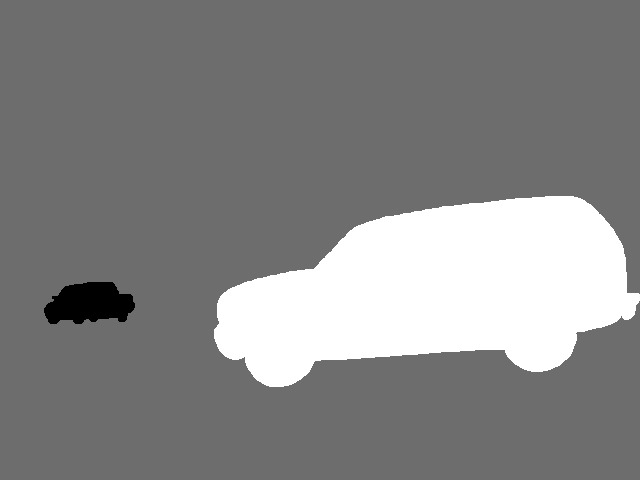
\includegraphics[width=0.47\linewidth] {implementation/merger/mask}
   \label{fig:merger_result_a}
}
\subfigure[Generated Segmentation]{
   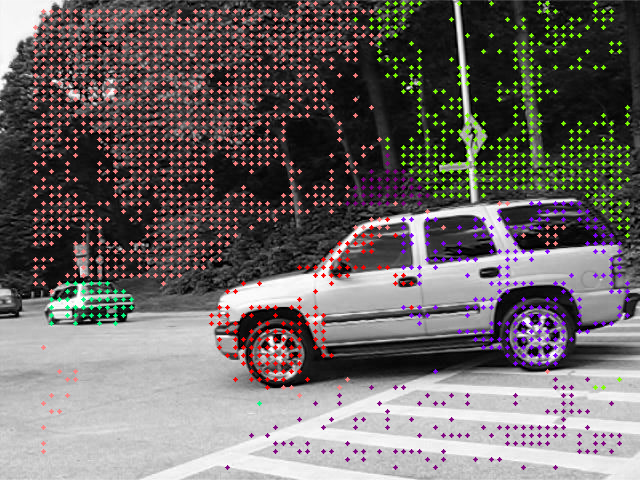
\includegraphics[width=0.47\linewidth] {implementation/merger/oversegmentation}
   \label{fig:merger_result_b}
}
~
\subfigure[Overlay Ground Truth / Segmentation]{
   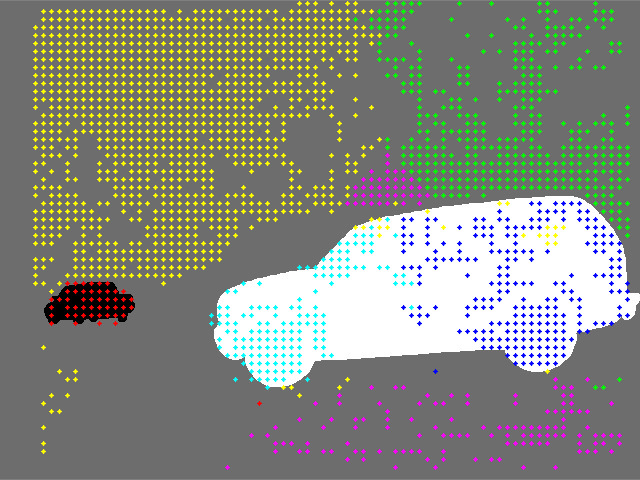
\includegraphics[width=0.47\linewidth] {implementation/merger/mask_segments_overlay}
   \label{fig:merger_result_c}
}
\subfigure[Merged Segmentation]{
   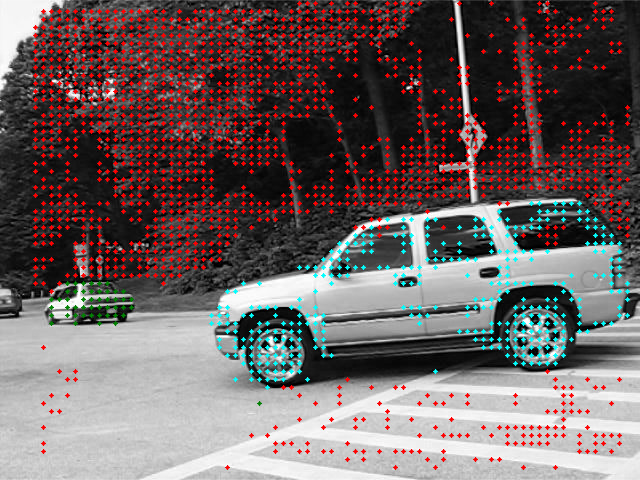
\includegraphics[width=0.47\linewidth] {implementation/merger/merged}
   \label{fig:merger_result_d}
}

\end{center}
\caption[Segmentation Merger]{Visualization of our segment merger's input and output. As an input it expects a ground truth segmentation (see figure $\ref{fig:merger_result_a}$) and a generated oversegmentation (see figure $\ref{fig:merger_result_b}$). As output it yields the merged segmentation as shown in subfigure $\ref{fig:merger_result_c}$.}
\label{fig:merger_result}
\end{figure}
Usually, the results generated by our pipeline exhibit an oversegmentation when comparing them against their ground truth. An example of such an oversegmentation is illustrated in figure $\ref{fig:merger_result_b}$. Ideally, before evaluating the quality, we would like to refine our over-segmented results in a way to reduce the total number of unnecessary segments. Therefore, we initially attempt to merge segments causing an oversegmentation of an ground truth mask. The goal of the merging phase is to lower the number of total segments but the same time retain meaningful segmentation labels. 

Conceptually, our merging approach is visualized in figure $\ref{fig:merger_result}$. Different approaches how to implement such a merging mechanism are described in literature (LIST SOME REFS HERE). However, we use a much simpler approach. 

A segmentation $S$ is basically a set of points in which every point is assigned to a certain segment identifier. In the following let us denote $S_j$ as the subset of points in $S$ that belong to the segmentation label $j$. Similarly, let $M$ denote the set of all ground truth points with their corresponding mask labels and $M_i$ the set of all points that belong to the ground truth mask $i$. To compute the merged segments we do the following: For every segment $S_j$ in $S$ we determine its best matching ground truth segment $M_i$ as defined in equation $\ref{eq:merging_label_formula}$. 
\begin{equation}
i = \argmaxl_{M_i \in M} \left\vert{S_j \cap M_i}\right\vert
\label{eq:merging_label_formula}
\end{equation}
The idea is to find the ground truth mask $i$ that yields the most point intersections with the currently considered segment $S_j$. Next, we update every point in $S_j$ by setting their segment label to $i$. After doing so we have computed the merged segmentation version of the initial oversegmentation. An example is shown in figure $\ref{fig:merger_result_c}$.

\section{Evaluation Program}
Finally, in this last section we describe how we evaluate our generated segmentations. Principally, the quality of a resulting segmentation is measured by comparing it against a manually drawn ground truth segmentation image.

\section{NOTES}
mention pipeline assumptions
discuss the details about each pipeline stage
mention in which language the individual parts are coded.
